\chapter{Optimization using local approximations}
The optimization problems in the previous chapters utilized explicit functions for the objective functions and constraints. However, in most practical structural optimization problems, we are not able to formulate such explicit functions. Instead, we use local approximations as a remedy. These should be explicit convex functions that approximate the structural problem in a local region well and are easy to solve at the same time. 

The procedure using a local approximation is as follows:

\begin{enumerate}
    \item Choose a starting point $\mathbf{x}^0$
    \item Evaluate the target function, constraints and their gradients at the current position $\mathbf{x}^k$.
    \item Construct a local, explicit, and convex approximation $\tilde{f}, \tilde{g}, \tilde{h}$ at $\mathbf{x}^k$.
    \item Solve the approximated optimization problem to find the next point $\mathbf{x}^{k+1}$. 
    \item Repeat steps 2, 3, and 4 until you reached a maximum number of iteration $k \le N$ or there is no improvement anymore.
\end{enumerate}

Note that during the optimization within each iteration, we use only the approximation and do not have to evaluate the expensive target function.

\begin{objectives}{}{objectives_approximation}
After studying this chapter and finishing the exercise, you should be able to 
\begin{itemize}[label=$\dots$]
    \item approximate an optimization problem via Sequential Linear Programming (SLP)
    \item approximate an optimization problem via Sequential Quadratic Programming (SQP)
    \item approximate an optimization problem via Convex Linearization (CONLIN)
    \item approximate an optimization problem via the Method of Moving Asymptotes (MMA)
    \item discuss the relation between these approximation methods and chose an appropriate method for a given task
\end{itemize}
\end{objectives}

\section{Sequential linear programming}
In Sequential Linear Programming (SLP), we approximate the functions in Equation \eqref{eq:constrained_optimization} at $\mathbf{x}^k$ with first order linear equations  
\begin{align}
    \tilde{f}(\mathbf{x}) &= f(\mathbf{x}^k) + \nabla f(\mathbf{x}^k) \cdot \left(\mathbf{x} - \mathbf{x}^k \right) \\
    \tilde{g}_i(\mathbf{x}) &= g_i(\mathbf{x}^k) + \nabla g_i(\mathbf{x}^k) \cdot \left(\mathbf{x} - \mathbf{x}^k \right) \\
    \tilde{h}_j(\mathbf{x}) &= h_j(\mathbf{x}^k) + \nabla h_j(\mathbf{x}^k) \cdot \left(\mathbf{x} - \mathbf{x}^k \right)
\end{align}
and limit the validity of the approximation with so-called \emph{move limits} 
\begin{equation}
    \tilde{\mathbf{x}}^{l,k} \le \mathbf{x}^k \le \tilde{\mathbf{x}}^{u,k}.
\end{equation}
The resulting functions are explicit linear expressions and the set for $\mathbf{x}$ is compact, hence the resulting problem is strictly convex. We limit the set because i) the approximation is only valid close to $\mathbf{x}^k$ and ii) the linear problem requires a compact set to be strictly convex. 

\begin{example}{SLP with move limits}{slpexample}
    We want to sequentially approximate the following quadratic function
    \begin{equation}
             f(\mathbf{x})= \mathbf{x} \cdot \mathbf{Q} \cdot \mathbf{x} \quad \text{with} \quad \mathbf{x} \in \mathcal{R}^2 \quad \text{and} \quad 
             \mathbf{Q} = 
            \begin{pmatrix}
            2 & 1 \\
            1 & 1 
            \end{pmatrix}. 
    \end{equation}
    Obviously, this is already an explicit convex function and we do not necessarily need to employ an approximation to minimize a function like this. But for the sake of this example, we assume that $f(\mathbf{x})$ is a very complex function with no explicit expression. 
    
    In this case we can get an explicit linear approximation
    \begin{align}
        \tilde{f}(\mathbf{x}) = f(\mathbf{x}^k) + 2(\mathbf{Q} \cdot \mathbf{x}^k) \cdot \left(\mathbf{x} - \mathbf{x}^k \right)
    \end{align}
    with an analytical expression for the gradient. Then, a first approximation at $\mathbf{x}^0=(1,1)^\top$ is 
    \begin{equation}
        \tilde{f}(\mathbf{x}) = 3 + \begin{pmatrix} 2\\1 \end{pmatrix} \cdot \left(\mathbf{x} - \mathbf{x}^k \right).
    \end{equation}
    Assuming a validity of $\pm 0.5$ around the approximated point, the move limits are $\tilde{\mathbf{x}}^{l,0}=(0.5, 0.5)^\top$ and  $\tilde{\mathbf{x}}^{u,0}=(1.5, 1.5)^\top$.  
    An optimization with these conditions yields to the next point $\mathbf{x}^1=(0.5,0.5)^\top$ with 
    \begin{equation}
        \tilde{f}(\mathbf{x}) = 1.25 + \begin{pmatrix} 1\\0.5 \end{pmatrix} \cdot \left(\mathbf{x} - \mathbf{x}^k \right)
    \end{equation}
    and with move limits $\tilde{\mathbf{x}}^{l,1}=(0, 0)^\top$ and  $\tilde{\mathbf{x}}^{u,1}=(1, 1)^\top$. 
    An optimization under these conditions gives us the final result $(0,0)^\top$ for the minimum of the function $f(\mathbf{x})$. We obtained this by sequentially employing linear approximations and then performing optimization on these approximations instead of the original "complex" and expensive function.
\end{example}

\section{Sequential quadratic programming}
In Sequential Quadratic Programming (SQP), we approximate the objective function in Equation \eqref{eq:constrained_optimization} at $\mathbf{x}^k$ with second order quadratic equations  
\begin{equation}
    \tilde{f}(\mathbf{x}) = f(\mathbf{x}^k) + \nabla f (\mathbf{x}^k) \cdot \left(\mathbf{x} - \mathbf{x}^k \right) + \left(\mathbf{x} - \mathbf{x}^k \right) \cdot \nabla^2 f(\mathbf{x}^k) \cdot \left(\mathbf{x} - \mathbf{x}^k \right)
\end{equation}
and the restrictions with first order linear approximations
\begin{align}
    \tilde{g}(\mathbf{x}) &= g(\mathbf{x}^k) + \nabla g(\mathbf{x}^k) \left(\mathbf{x} - \mathbf{x}^k \right) \\
    \tilde{h}(\mathbf{x}) &= h(\mathbf{x}^k) + \nabla h(\mathbf{x}^k) \left(\mathbf{x} - \mathbf{x}^k \right).
\end{align}
This results in a more accurate approximation and also in a more balanced approximation, i.e. the same approximation order for the roots of interest (for constraints we are interested in roots of the function itself, for the objective we are interest in the roots of the derivative). 
The Hessian $\nabla^2 f$ may be approximated efficiently using the BFGS algorithm. This way, the problem is convex and we may use the methods from Chapter 3 to obtain the optimum. 

\section{Convex linearization}
Both, SLP and SQP, can be applied for any non-linear optimization problem. However, we can improve the approximation quality significantly, if we leverage some knowledge about the fundamental equation types seen in structural optimization.

Let's consider an assembly of beams and design variables that describe the cross sectional areas of the beams like in the last example of Exercise 3. A property like volume or mass is linearly related to the design variables and a linear approximation would be exact. Conversely, stress and displacement are related to the inverse of the design variable and we would need many sequential linear approximations to approximate the inverse.  However, this knowledge suggests that it would be clever to substitute $y_j = x^{-1}_j$, which would lead to a exact approximations for statically determined truss assemblies \cite{Christensen2008}. 
%The notation $\bullet_j$ is used here for element-wise operations, i.e. double indices of this type do not imply a summation according to Einstein's summation convention. 
Then, our linear approximation becomes 
\begin{equation}
    \tilde{f}(\mathbf{x}) = f(\mathbf{x}^k) + \sum_j \frac{\partial f}{\partial y_j}(\mathbf{x}^k) \left(y_j(x_j) - y_j(x^k_j) \right)
\end{equation}
for the objective function, but obviously the same principals apply for constraints throughout the remainder of this chapter.
Employing the chain rule
\begin{equation}
    \frac{\partial f}{\partial y_j} (\mathbf{x}^k) 
    = \frac{\partial x_j}{\partial y_j} \frac{\partial f}{\partial x_j} (\mathbf{x}^k)   
    = -x^2_j \frac{\partial f}{\partial x_j}(\mathbf{x}^k) 
\end{equation}
this can be simplified to an expression without $y_j$
\begin{equation}
    \tilde{f}(\mathbf{x}) = f(\mathbf{x}^k) + \sum_j \frac{\partial f}{\partial x_j}(\mathbf{x}^k) \underbrace{\frac{x^k_j}{x_j}}_{\Gamma_j} \left(x_j - x^k_j \right). 
\end{equation}
The difference to the regular linear approximation is only the term indicated with $\Gamma_j$. Hence we can set $\Gamma_j = 1$ for variables that should be approximated linearly and set $\Gamma_j = x^k_j / x_j$ for variables that should be approximated inversely. Instead of choosing the approximation for each variable manually, we may use the the sign of the partial derivative and define an approximation method as 
\begin{align}
    \tilde{f}(\mathbf{x}) &= f(\mathbf{x}^k) + \sum_j \frac{\partial f}{\partial x_j}(\mathbf{x}^k) \Gamma_j \left(x_j - x^k_j \right) \\
    \Gamma_j &= 
    \begin{cases}
        1 &\quad \text{if} \quad \frac{\partial f}{\partial x_j} (\mathbf{x}^k) \ge 0 \\
        \frac{x^k_j}{x_j} &\quad \text{if} \quad \frac{\partial f}{\partial x_j} (\mathbf{x}^k) < 0.
    \end{cases}
\end{align}
This method is termed \emph{Convex Linearization} or CONLIN \cite{Fleury1989}. The CONLIN method provides a convex separable optimization problem, hence the Lagrangian duality method is a suitable solution method  \cite{Christensen2008,Harzheim2014}.

\begin{example}{CONLIN}{conlinexample}
    The volume of a four-bar truss \cite{Christensen2008} should be minimized under the displacement constraint $\delta \le \delta_0$. There is a force $P>0$ and all bars have identical lengths $l$ and identical Young's moduli $E$. The modifiable structural variables are the cross sectional areas $A_1=A_4$ and $A_2=A_3$. We define $A_0 = Pl / (10\delta_0E)$ and constrain the variables $0.2A_0 \le A_j \le 2.5 A_0$. Then we can use dimensionless design variables $a_1=A_1/A_0 \in [0.2, 2.5]$ and $a_2=A_2/A_0 \in [0.2, 2.5]$.
    \begin{center}
        
\includegraphics[width=0.8\textwidth]{figures/four_bar_truss_transparent.png}
    \end{center}
    The optimization problem is 
    \begin{equation}
        \begin{aligned}
            \min_{\mathbf{a}} \quad & f(\mathbf{a})= a_1 + a_2\\
            \textrm{s.t.} \quad     & g(\mathbf{a}) = \frac{8}{16a_1+9a_2} - \frac{4.5}{9a_1+16a_2} -0.1 \le 0  \\
            \quad     & \mathbf{a} \in [0.2,2.5]^2
        \end{aligned}
    \end{equation}
    This problem is not convex, because the constraint $g(\mathbf{a})$ (shown as solid black line in the following plot) is not a convex function. This leads to two local minima, one at $a_2=0.2$ and one at $a_2=2.5$.
    \begin{center}
        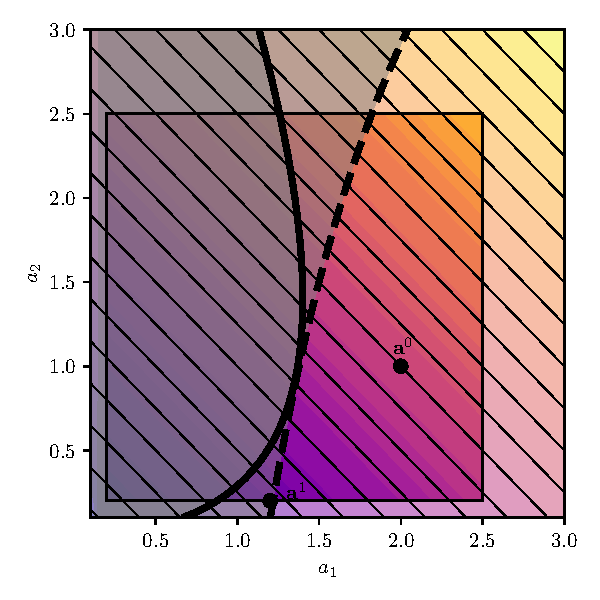
\includegraphics[width=0.6\textwidth]{figures/four_bar_example_0.pdf}
    \end{center}
    
    The CONLIN approximation of the objective function is the objective function itself - it is already linear. A CONLIN approximation of the constraint function at $\mathbf{a}^0=(2,1)^\top$ is computed using automatic differentiation in PyTorch and results in the dashed black line. The resulting problem is convex and can be solved, e.g. using Lagrangian duality. The unique solution of this problem is the point $\mathbf{a}^1=(1.2,0.2)^\top$. We can apply the CONLIN method again at this point to obtain a new convex problem. Solving this problem gives $\mathbf{x}^2=(0.85,0.2)^\top$, which is close to the optimal solution $\mathbf{a}^*$, but could be improved with further iterations. Note that not every CONLIN approximation is conservative, i.e. it can happen that $\tilde{g}(\mathbf{a}) < g(\mathbf{a})$. In that case, the solution will tend to oscillate around the optimal point. 
    \begin{center}
        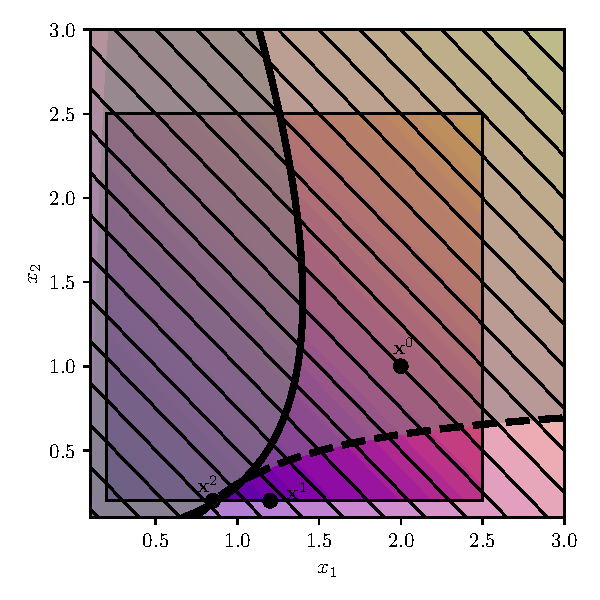
\includegraphics[width=0.6\textwidth]{figures/four_bar_example_1.pdf}
    \end{center}
\end{example}

\section{Method of Moving Asymptotes}
CONLIN is an effective method to turn structural optimization problems into convex separable optimization tasks. However, it is sometimes too conservative causing slow convergence or sometimes not conservative enough causing no convergence at all. We could improve the method by adjusting how conservative we approximate a function.

We may obtain an adjustable method by defining
\begin{equation}
    \tilde{f}(\mathbf{x}) = r(\mathbf{x}^k) + \sum_j \frac{p_{j}^k}{U^k_j-x_j} + \frac{q_{j}^k}{x_j-L^k_j} 
    \label{eq:mma_start}
\end{equation}
where
\begin{align}
    p_{j}^k &= 
    \begin{cases}
        (U^k_j-x^k_j)^2 \frac{\partial f}{\partial x_j} (\mathbf{x}^k)  &\quad \text{if} \quad \frac{\partial f}{\partial x_j} (\mathbf{x}^k) > 0 \\
        0 &\quad \text{if} \quad \frac{\partial f}{\partial x_j} (\mathbf{x}^k) \le 0.
    \end{cases} \\ 
    q_{j}^k &= 
    \begin{cases}
         0 &\quad \text{if} \quad \frac{\partial f}{\partial x_j} (\mathbf{x}^k) \ge 0 \\
        - (x^k_j-L^k_j)^2 \frac{\partial f}{\partial x_j} (\mathbf{x}^k) &\quad \text{if} \quad \frac{\partial f}{\partial x_j} (\mathbf{x}^k) < 0.
    \end{cases} \\ 
    r_j^k &= f(\mathbf{x}^k) - \sum_j \frac{p_{j}^k}{U^k_j-x^k_j} + \frac{q_{j}^k}{x^k_j-L^k_j} 
    \label{eq:mma_end}
\end{align}
with $L^k_j < x_j < U^k_j$. The parameters $L^k_j$ and $U_j^k$ are called the lower and upper asymptotes, respectively. They can be adjusted ("move"), hence the method is termed \emph{Method of Moving Asymptotes} (MMA) \cite{Svanberg1987}. It can be proven that this is a generalization, as setting $L^k_j \rightarrow 0$ and $U^k_j \rightarrow \infty$ recovers the CONLIN method and setting  $L^k_j \rightarrow -\infty$ and $U^k_j \rightarrow \infty$ recovers the SLP method.

To prevent singularities by reaching the asymptotes, we use move limits 
\begin{equation}
    L^k_j \le \tilde{x}_j^{l,k} \le x_j^{l,k} \le \tilde{x}_j^{u,k} \le U_j^k.
\end{equation}
similar to SLP. These could be chosen for example as 
\begin{align}
    \tilde{x}_j^{l,k} &= \max(x_j^l,  0.9 L_j^k + 0.1 x_j^k) \\
    \tilde{x}_j^{u,k} &= \min(x^u_j, 0.9 U_j^k + 0.1 x_j^k).
\end{align}

The advantage of these adjustable asymptotes is that we can bring the asymptotes closer to the current approximation $\mathbf{x}^k$ to obtain a more conservative approximation and move them further away to accelerate convergence speed. But how do we chose the asymptotes? Svanberg \cite{Svanberg1987} suggested the following heuristic approach: 
\begin{enumerate}
    \item In the first two iterations, set 
        \begin{align}
            L_j^k &= x_j^k - s_0 (x^u_j - x^l_j) \\
            U^k_j &= x_j^k + s_0 (x^u_j - x^l_j)
        \end{align}
    with $s_0 \in (0,1)$.
    \item For the following iterations ($k>1$) check for each design variable, if it oscillates. If it oscillates, i.e. $(x_j^k-x_j^{k-1})(x_j^{k-1}-x_j^{k-2}) < 0$, bring asymptotes closer to $x_j^k$ by   
        \begin{align}            
            \label{eq:mma_heuristic_first}
            l_j^k &= x_j^k - s (x_j^{k-1} - l_j^{k-1}) \\
            u_j^k &= x_j^k + s (u_j^{k-1} - x_j^{k-1})
        \end{align}
    with $s \in (0,1)$. 

    If the solution does not oscillate, i.e. $(x_j^k-x_j^{k-1})(x_j^{k-1}-x_j^{k-2}) \ge 0$, move the asymptotes further away from $x_j^k$ by   
        \begin{align}
            l_j^k &= x_j^k - \frac{1}{\sqrt{s}} (x_j^{k-1} - l_j^{k-1}) \\
            u_j^k &= x_j^k + \frac{1}{\sqrt{s}} (u_j^{k-1} - x_j^{k-1}).
            \label{eq:mma_heuristic_last}
        \end{align}
\end{enumerate}

Svanbergs original version uses the same asymptotes $L_j^k$ and $U_j^k$ for the objective function and constraints. There is also a method termed \emph{Generalized Method of Moving Asymptotes} (GMMA) \cite{Zhang1997} that uses different asymptotes for each function. However, this requires a more complicated heuristic to obtain such asymptotes.

\begin{example}{MMA}{mmaexample}
    Consider the previous example with the optimization problem
    \begin{equation}
        \begin{aligned}
            \min_{\mathbf{a}} \quad & f(\mathbf{a})= a_1 + a_2\\
            \textrm{s.t.} \quad     & g(\mathbf{a}) = \frac{8}{16a_1+9a_2} - \frac{4.5}{9a_1+16a_2} -0.1 \le 0  \\
            \quad     & \mathbf{a} \in [0.2,2.5]^2
        \end{aligned}
    \end{equation}

    A MMA approximation at $\mathbf{a}^0=(2,1)^\top$ is illustrated in the following image with the dashed line for $s_0=0.2$. 
    \begin{center}
        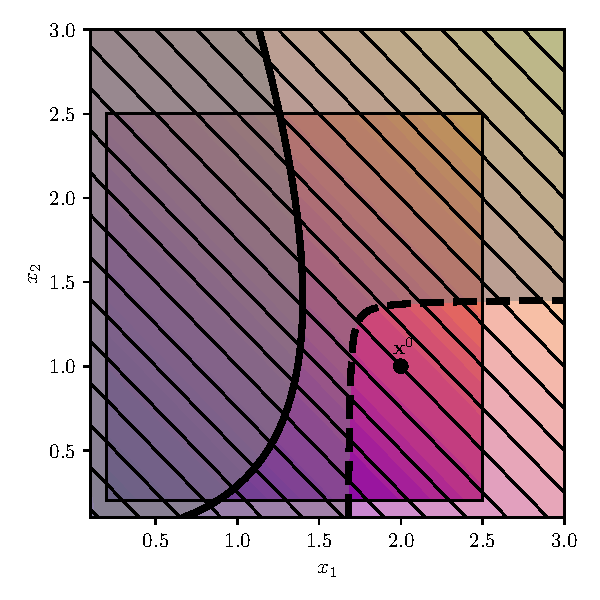
\includegraphics[width=0.6\textwidth]{figures/four_bar_example_mma_0.pdf}
    \end{center}

    If we chose $s_0=0.5$, we get a less conservative approximation, as shown in the next image. This results in faster convergence, as an optimization of the convex problem gets closer to the optimum in a single step.
    \begin{center}
        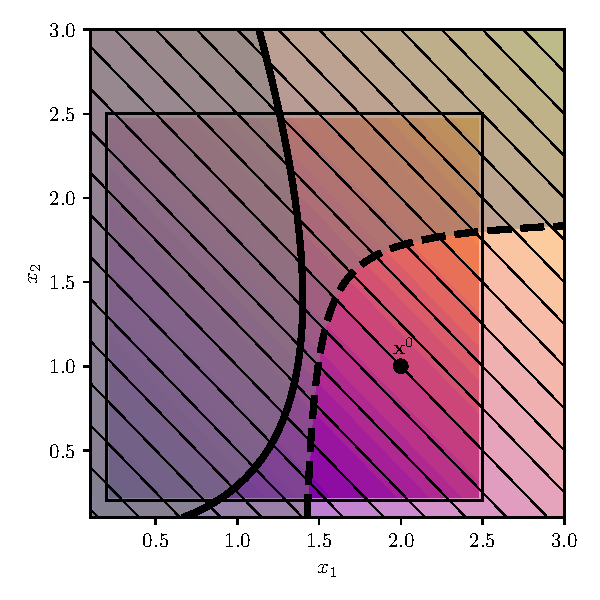
\includegraphics[width=0.6\textwidth]{figures/four_bar_example_mma_1.pdf}
    \end{center}

    This example shows just the first iteration - the full method would require sequential approximation and optimization with the Lagrangian duality method until convergence. During each iteration, we would use the heuristic given in Equations \eqref{eq:mma_heuristic_first} to \eqref{eq:mma_heuristic_last} to update asymptotes.  
\end{example}

\bibliographystyle{unsrtnat}
\bibliography{literature} 